%%%%%%%%%%%%%%%%%%%%%%%%%%%%%%%%%%%%%%%%%%%%%%%%%%%%%%%%%%%%%%%%%
% Project:  A Format Selection Framework for AI Agent Data Transmission
% Template: VLDB 2020-08-03 (ACM 1.7.0)
%%%%%%%%%%%%%%%%%%%%%%%%%%%%%%%%%%%%%%%%%%%%%%%%%%%%%%%%%%%%%%%%%

\documentclass[sigconf, nonacm]{acmart}

%% BibTeX command
\AtBeginDocument{%
  \providecommand\BibTeX{{%
    \normalfont B\kern-0.5em{\sc i\kern-0.25em b}\kern-0-8em\TeX}}}

%% Packages
\usepackage{subcaption}
\usepackage{cleveref}
\usepackage{algorithm}
\usepackage{algpseudocode}
\usepackage{array}
\usepackage{xcolor}

% --- Custom Commands ---
\newcommand\todo[1]{\textcolor{red}{#1}}

% === SYSTEM NAME ===
\newcommand{\system}{TransForm} 

% Highlighted block for instructor notes/feedback
\newcommand{\highlight}[1]{\colorbox{yellow}{\parbox{\dimexpr\columnwidth-2\fboxsep\relax}{#1}}}

%% VLDB Metadata (Updated for 2026)
\newcommand\vldbdoi{10.14778/xxxxxxx.xxxxxxx}
\newcommand\vldbpages{XXX-XXX}
\newcommand\vldbvolume{19}
\newcommand\vldbissue{1}
\newcommand\vldbyear{2026}
\newcommand\vldbauthors{\authors}
\newcommand\vldbtitle{\shorttitle}
\newcommand\vldbavailabilityurl{https://github.com/YourRepo/TransForm}
\newcommand\vldbpagestyle{plain}

\begin{document}

\title{\system: A Dynamic Format Selection Framework for Data Transmission in AI Agent Systems}

%% AUTHOR UPDATES
%% AUTHOR UPDATES
\author{Shashank Mukkera}
\affiliation{%
  \institution{Purdue University}
  % \city{West Lafayette}
  % \state{Indiana}
  \country{USA}
}
\email{smukkera@purdue.edu}

\author{Chunwei Liu}
\affiliation{%
  \institution{Purdue University}
  % \city{West Lafayette}
  % \state{Indiana}
  \country{USA}
}
\email{chunwei@purdue.edu}

\begin{abstract}
Model Context Protocol (MCP) is emerging as a ``REST API for AI agents,'' standardizing how models call tools and consume structured results. However, MCP’s control plane is JSON-RPC, and JSON is structurally inefficient for large tabular tool outputs: it inflates payload bytes, stresses context budgets, and blocks incremental consumption. We present \system, a control/data-plane split for MCP tool results. Tools return a small MCP response (a \texttt{CallToolResult} envelope) containing human-readable text plus a machine-readable descriptor that points to a data plane served over streamable HTTP. For large tables, the data plane delivers Parquet either as a whole blob or as a length-prefixed chunk stream, enabling time-to-first-rows, early termination, and bounded client memory. \system includes a format-selection framework that uses optimization targets (min bytes, min latency, or min time-to-first-rows), server-provided size hints, and optional online bandit learning; within the Parquet arm it can also choose codecs/encodings.\ We evaluate on (i) controlled synthetic grids and TPC-DS \texttt{catalog\_sales} slices to characterize size scaling and decode proxies, and (ii) BIRD dev SQLite query results to measure real workload distributions. On synthetic grids, JSON transfers are 2.7--2.9$\times$ larger than Parquet blobs. On BIRD full dev (1534 queries), hint-aware selection reduces aggregate wire volume from 43.4\,MB (JSON baseline) to 6.4\,MB (6.8$\times$), while preserving millisecond-scale localhost fetch latency; the additional ``describe'' round-trip can be avoided with a one-shot server-side selector. These results suggest that separating MCP control from a tabular data plane is a practical path to scalable agent-first data access.
\end{abstract}

\maketitle

%%% VLDB block start %%%
\pagestyle{\vldbpagestyle}
\begingroup\small\noindent\raggedright\textbf{PVLDB Reference Format:}\\
\vldbauthors. \vldbtitle. PVLDB, \vldbvolume(\vldbissue): \vldbpages, \vldbyear.\\
\href{https://doi.org/\vldbdoi}{doi:\vldbdoi}
\endgroup

\begingroup
\renewcommand\thefootnote{}\footnote{\noindent
This work is licensed under the Creative Commons BY-NC-ND 4.0 International License. Visit \url{https://creativecommons.org/licenses/by-nc-nd/4.0/} to view a copy of this license. Publication rights licensed to the VLDB Endowment. \\
\raggedright Proceedings of the VLDB Endowment, Vol. \vldbvolume, No. \vldbissue\ %
ISSN 2150-8097. \\
\href{https://doi.org/\vldbdoi}{doi:\vldbdoi} \\
}\addtocounter{footnote}{-1}\endgroup
%%% VLDB block end %%%

\section{Introduction}
\label{sec:intro}

AI agents are increasingly deployed as tool-using systems: they issue queries, call APIs, manipulate files, and iterate over intermediate results in plan--act--reflect loops. Model Context Protocol (MCP) is emerging as an interoperability layer for this ecosystem, standardizing a JSON-RPC control plane with primitives such as tools, resources, prompts, and notifications. MCP resembles a ``REST API for AI,'' but it is fundamentally message-oriented: tool inputs and outputs become part of the agent’s working memory and often flow through model context. As a result, the bottleneck for many tool-augmented workflows shifts from computation to \emph{data transmission} and \emph{representation} of tool outputs.

\smallskip
\noindent\textbf{Motivation: large structured tool outputs.}
A common pattern is text-to-SQL and analytics tools that return tabular query results. In today’s MCP deployments, these results are frequently encoded directly as JSON objects (e.g., lists of records) and returned through the MCP control plane. JSON is convenient and widely supported, but it is structurally inefficient for tables: it repeats column names, inflates bytes, and forces clients (and models) to receive the entire payload before acting. In agentic workloads, this is particularly costly: agents often do not need the full table to proceed, and they benefit from time-to-first-rows and the ability to terminate early when confidence is sufficient.

\smallskip
\noindent\textbf{MCP layering and deployment realities.}
MCP consists of (i) a \emph{data layer} that defines JSON-RPC lifecycle and core primitives, and (ii) a \emph{transport layer} that defines how messages flow (e.g., local STDIO vs.\ remote streamable HTTP). Local MCP servers that use STDIO typically serve a single client process, while remote MCP servers over streamable HTTP are designed to serve many clients and must account for authorization, payload limits, and fairness. These realities motivate a separation between the control plane (small JSON-RPC messages) and a data plane optimized for large artifacts.

\smallskip
\noindent\textbf{Our approach.}
We present \system, a dynamic format selection framework for MCP tool outputs that separates \emph{control} from \emph{data}. Tools return a small \texttt{CallToolResult} envelope with (a) concise natural language and (b) structured descriptors describing how to fetch and decode large results. Large structured outputs are delivered on a streamable HTTP data plane using Parquet as a binary columnar representation, either as a whole blob or as a length-prefixed chunk stream. This design supports incremental client processing, bounded memory, and early termination; it also accommodates other encodings (e.g., Arrow IPC) and unstructured payloads.

\smallskip
\noindent\textbf{Format selection.}
\system selects among output formats based on an explicit optimization target (min bytes, min latency, or min time-to-first-rows). Selection can be client-driven (using server-provided size hints) or server-driven (one-shot selection inside a single MCP tool), and it can be extended with online learning (multi-armed bandits) and codec/encoding choices within Parquet.

\smallskip
\noindent\textbf{Contributions.}
This paper makes the following contributions:
\begin{itemize}
    \item \textbf{Control/data-plane split for MCP results.} We define a descriptor-based interface that keeps MCP JSON-RPC messages small while delivering large tabular payloads via a streamable HTTP data plane.
    \item \textbf{Parquet blob and Parquet chunk streaming for tool outputs.} We implement both whole-blob delivery and incremental, length-prefixed chunk streaming to enable low time-to-first-rows and early termination.
    \item \textbf{Dynamic format (and codec) selection.} We design a target-driven selector using size hints and optional network+decode proxies, and we support both client-side and one-shot server-side selection.
    \item \textbf{Evaluation on controlled and real workloads.} We quantify size scaling on TPC-DS slices and measure payload and latency behavior on BIRD dev query results, demonstrating substantial reductions in aggregate wire volume versus JSON baselines.
\end{itemize}

\smallskip
\noindent\textbf{Paper roadmap.}
Section~\ref{sec:related} discusses related work. Section~\ref{sec:overview} presents \system’s architecture, protocols, and selectors. Section~\ref{sec:eval} evaluates payload and latency trade-offs on TPC-DS and BIRD. Section~\ref{sec:conclude} concludes with limitations and future directions.

\section{Related Work}
\label{sec:related}

This section summarizes related work on (i) MCP ecosystems and tool interoperability, (ii) agentic workloads and ``agent-first'' data systems, and (iii) data formats and adaptive representation/selection for tabular results.

\subsection{MCP ecosystem and tool protocols}
MCP standardizes how AI clients call tools and consume results through a JSON-RPC data layer and multiple transports. A recent measurement study of the MCP ecosystem highlights that MCP is already deployed at scale but remains heterogeneous and fragile, with many low-quality listings and an under-adoption of scalable transports in clients \cite{guoMcpEcosystemMeasurement}. These findings motivate systems-level work on robust, scalable handling of tool outputs and response formats. \system complements MCP’s control plane by introducing a tabular data plane for large structured results while remaining backward-compatible with JSON-only clients.

\subsection{Agentic workloads and agent-first data systems}
Recent work argues that LLM agents will become dominant ``users'' of data systems and that their workloads exhibit high throughput, redundancy, and a need for rapid iteration (``agentic speculation'') \cite{liuAgentFirstOverlords}. Industry perspectives similarly emphasize that agent success degrades sharply when latency increases beyond a few seconds and call for standards-based integration with existing data stacks \cite{fireboltAgentsWhitepaper}. Our work is orthogonal to query execution optimizations inside the database: we focus on the representation and delivery of tool results across the control/data boundary, which becomes a bottleneck as agents iterate.

\subsection{Data formats for analytical systems}
Columnar formats such as Parquet and Arrow are widely used for analytical workloads and interchange. A recent survey of data formats in analytical DBMSs characterizes trade-offs among Arrow, Parquet, and ORC, noting that Parquet typically provides strong compression and I/O efficiency while Arrow provides fast in-memory interchange \cite{liuDataFormatsVldbj2025}. We leverage these established trade-offs to motivate a Parquet-based data plane for large tabular tool outputs while treating Arrow IPC as a reference point when decode speed dominates.

\subsection{Adaptive representation and efficiency of structured outputs}
Several lines of work motivate going beyond ``always JSON''. Byte-level analyses show that text-based encodings can reduce redundancy for tabular structures compared to generic JSON \cite{toonVsJsonModel}. More broadly, adaptive, input-dependent selection among methods---including online explore/exploit policies---has been studied in the context of dynamic compression selection \cite{adaedge}. \system applies this lens to tool-result delivery: it selects among JSON, Parquet blob, and streaming formats based on explicit optimization targets and measurable hints, and it extends selection within Parquet via codec/encoding choices.

\subsection{Table reasoning agents and tool-augmented execution}
Strong table reasoning increasingly relies on programmatic backends and tool use, including code-generation loops that execute computations over tables \cite{tablemindWsdm2026}. These systems amplify the importance of efficient tool-result delivery: as agents issue many exploratory queries, the cost of transferring large intermediate tables can dominate end-to-end performance. \system provides a compatible substrate for such tool-augmented table workflows by optimizing how tabular results are delivered and consumed.

\section{Overview}
\label{sec:overview}

This section describes \system’s architecture and the mechanisms used to deliver large tool outputs efficiently while remaining compatible with MCP’s JSON-RPC control plane.

\subsection{Background: MCP layers and deployment}
MCP consists of two layers. The \textbf{data layer} defines the JSON-RPC protocol and lifecycle management, and the core primitives that clients and servers offer each other: tools (callable functions), resources (addressable data), prompts, and notifications. The \textbf{transport layer} defines the channel for exchanging JSON-RPC messages. In practice, MCP is deployed over either (i) a local STDIO transport, typically serving a single client, or (ii) a remote streamable HTTP transport, typically serving many clients. Streamable HTTP uses HTTP POST for client-to-server messages and may use Server-Sent Events (SSE) for streaming model-facing updates; it also provides a natural hook point for authorization and payload controls.

\subsection{Control plane vs.\ data plane}
\system addresses the mismatch between MCP’s control plane and large structured payloads by splitting responsibilities:
\begin{itemize}
    \item \textbf{Control plane (MCP JSON-RPC).} Tool calls return a small \texttt{CallToolResult} envelope containing: (i) a short natural-language summary suitable for UIs and models, and (ii) a machine-readable \emph{descriptor} that tells the client how to retrieve and decode the full payload.
    \item \textbf{Data plane (HTTP).} Large payload bytes are delivered over HTTP endpoints as either a whole blob or a stream. This keeps MCP messages small, enables incremental consumption, and avoids pushing large tables into model context.
\end{itemize}

\subsection{Payload kinds and decode descriptors}
\system treats outputs as one of two payload kinds:
\begin{itemize}
    \item \textbf{Tabular payloads}: data frames / result tables.
    \item \textbf{Unstructured payloads}: text or arbitrary bytes (e.g., files, images, logs).
\end{itemize}

For tabular payloads, the descriptor returned in \texttt{structured\_content} specifies the chosen representation and how to decode it. Concretely, the descriptor includes a \texttt{decode} object with:
\begin{itemize}
    \item \textbf{\texttt{decode.transport}}: \texttt{inline} (no HTTP), \texttt{http\_blob} (download full object), or \texttt{http\_length\_prefixed\_stream} (consume a stream of chunks).
    \item \textbf{\texttt{decode.encoding}}: \texttt{json\_records}, \texttt{parquet}, or \texttt{arrow\_ipc}.
\end{itemize}
Unstructured payloads follow the same pattern: small text may be returned inline, while large bytes are referenced by URL (optionally compressed).

\subsection{Tabular formats}
\system supports multiple arms for large tabular results:
\begin{itemize}
    \item \textbf{JSON records (baseline).} The result table is serialized as a list of JSON dictionaries. This is the default compatibility path for existing MCP clients and for small results.
    \item \textbf{Parquet blob.} The result table is encoded as a single Parquet file and served via a \texttt{GET} endpoint. Parquet is typically the smallest on the wire due to columnar layout and compression.
    \item \textbf{Parquet stream.} The result table is partitioned into row chunks (e.g., fixed rows-per-chunk). The server emits a length-prefixed byte stream so the client can fetch, decode, and process chunks incrementally. This optimizes time-to-first-rows and enables early termination.
    \item \textbf{Arrow IPC (optional).} Arrow IPC can be used when client stacks benefit from fast in-memory interchange. In our evaluation we use Arrow IPC mainly as a reference point for decode-speed trade-offs.
\end{itemize}

\subsection{Format selection}
\system chooses a representation based on an explicit \textbf{optimization target}:
\texttt{min\_bytes}, \texttt{min\_latency}, or \texttt{min\_time\_to\_first\_rows} (TTFR). We support two selection placements.

\smallskip
\noindent\textbf{Workflow A (client-driven).}
The client calls a hint tool (e.g., \texttt{describe\_result\_formats}) to obtain approximate byte sizes for candidate encodings (JSON, Parquet, Arrow IPC; plus first-chunk sizes for streaming). Given the hints and target, the client runs a deterministic selector to choose which tool variant to call (JSON vs.\ Parquet blob vs.\ stream).

\smallskip
\noindent\textbf{Server-side one-shot selection.}
To remove the extra hint round-trip, the server can expose a single MCP tool (e.g., \texttt{large\_result\_auto}) that accepts an optimization target and returns a descriptor whose \texttt{chosen\_format} and \texttt{decode} fields fully specify the selected arm. Fetching bytes may still occur on the HTTP data plane, but no additional MCP call is required.

\smallskip
\noindent\textbf{Latency proxy model.}
For \texttt{min\_latency}, selection can optionally incorporate a simple model that combines transfer time under an assumed bandwidth with a decode proxy measured as nanoseconds per byte (calibrated empirically on representative slices). This allows the selector to trade off Parquet’s smaller bytes against Arrow IPC’s faster decode in Arrow-native clients.

\subsection{Codec and encoding selection within Parquet}
Within the Parquet arms, \system can select compression codecs (e.g., Snappy, Zstd, Gzip) and optional column encodings based on a target-driven policy. While Parquet often minimizes wire bytes compared to JSON, codec choice further trades off size versus encode+decode time. Our evaluation includes a first pass at characterizing this Pareto frontier for TPC-DS-derived tables.

\subsection{Implementation overview}
We implement \system as a Python MCP server that serves both the JSON-RPC control plane and the HTTP data plane. For tabular results we use \texttt{pandas} for in-process materialization and \texttt{pyarrow} for Parquet (and Arrow IPC) encoding/decoding. The client benchmarks materialize SQL results locally (for BIRD), register them once, then compare baseline JSON transport to hint-aware selection and one-shot server-side selection on the same materialized result id.

\section{Evaluation}
\label{sec:eval}

This section evaluates \system’s impact on (i) wire payload size, (ii) time-to-first-rows (TTFR) for streaming, (iii) end-to-end transport latency on a real NL2SQL benchmark workload with fixed SQL, and (iv) codec trade-offs within Parquet. Full recorded runs and reproduction commands are included in the project artifacts.

\subsection{Experimental setup}
\noindent\textbf{Server and protocols.}
We run a local MCP server that exposes a JSON-RPC control plane and an HTTP data plane. The baseline arm returns tabular tool outputs as JSON records through MCP. The enhanced arm returns a descriptor through MCP and delivers the bytes via HTTP as either a Parquet blob or a length-prefixed Parquet chunk stream; it may additionally call \texttt{describe\_result\_formats} to obtain size hints, unless using one-shot server-side selection.

\smallskip
\noindent\textbf{Datasets.}
We use (i) synthetic grids with controlled \((n\_rows, n\_cols)\), (ii) TPC-DS \texttt{catalog\_sales} slices to characterize format scaling and decode proxies, and (iii) BIRD dev query results (SQLite port) to evaluate transport on real workloads while controlling for NL2SQL.

\smallskip
\noindent\textbf{Metrics.}
We report \textbf{bytes} (payload size on the wire), \textbf{fetch latency} (baseline JSON fetch vs.\ enhanced single fetch), \textbf{describe+fetch latency} (client-driven selection overhead), and a TTFR proxy for streaming using first-chunk bytes and time-to-first-chunk decode. On BIRD we emphasize p95 and \textbf{aggregate sums of bytes} across the split, since median results are often tiny.

\subsection{Format size scaling on TPC-DS slices}
Figure~\ref{fig:tpcdsSizeScaling} shows payload bytes as a function of rows for representative column counts. Parquet consistently yields the smallest wire sizes, while Arrow IPC is intermediate and JSON is largest. This behavior matches the expected inefficiency of JSON for tabular layouts (repeated keys, string overhead), and it motivates keeping large tables out of MCP message bodies.

\begin{figure}[t]
  \centering
  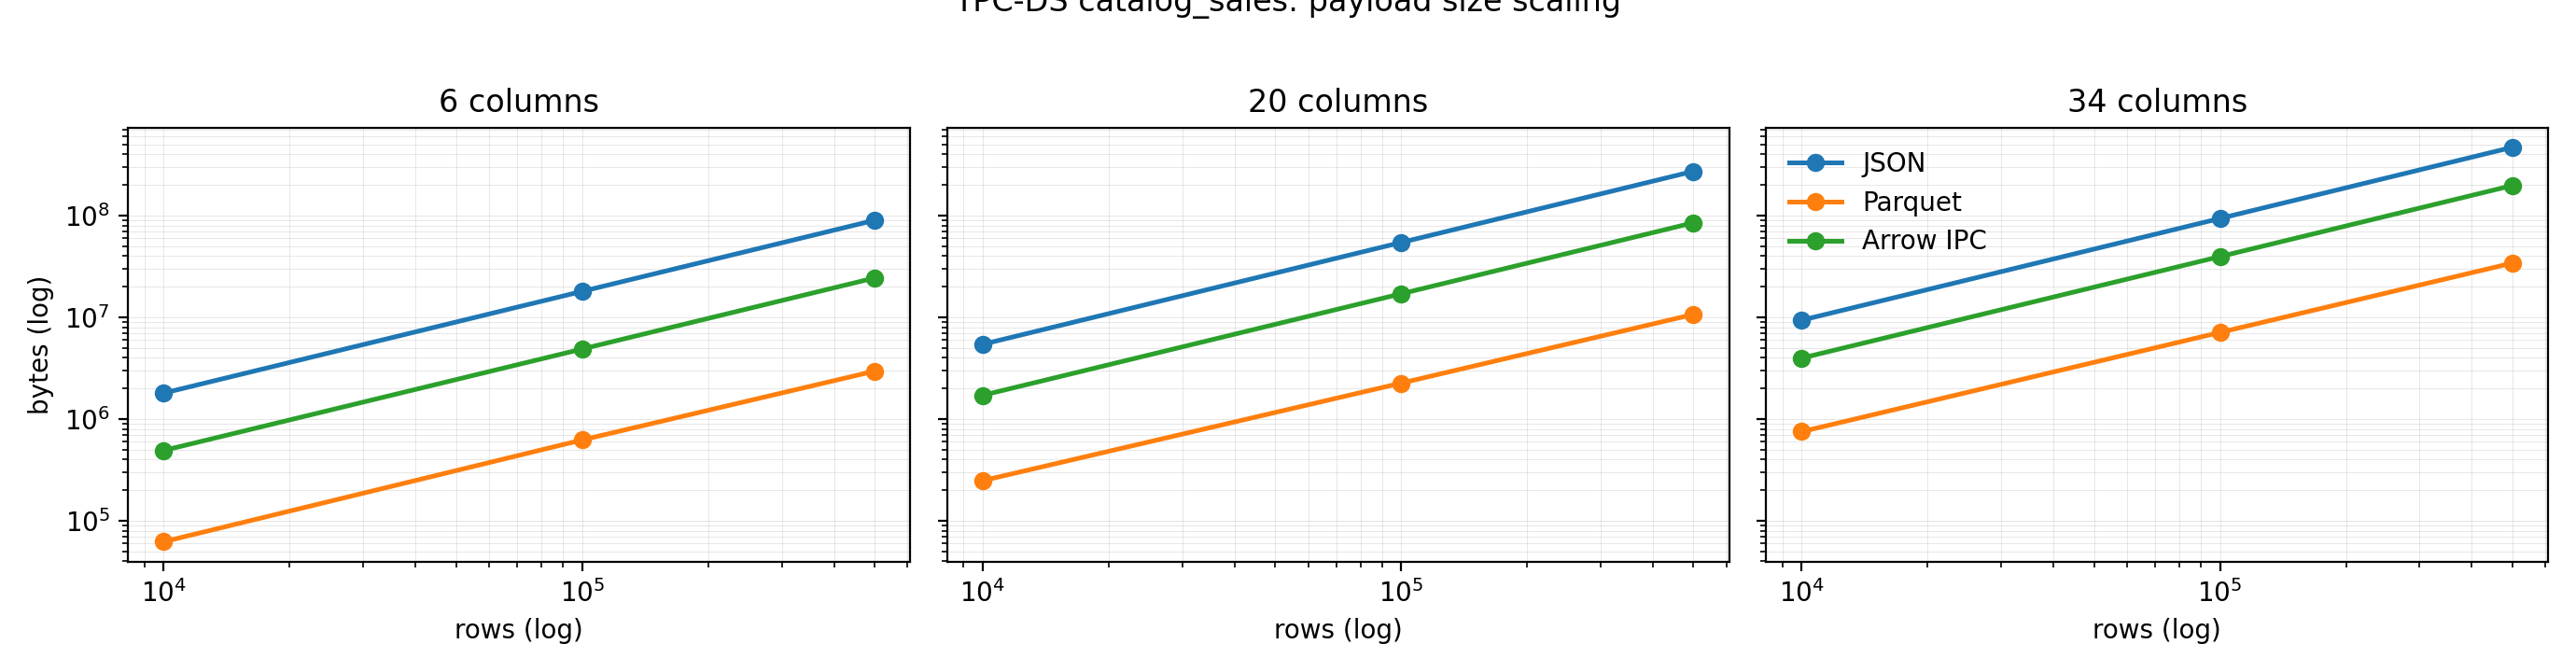
\includegraphics[width=\columnwidth]{figures/fig_A1_tpcds_size_scaling.png}
  \Description{Log-scale line plots showing how payload bytes scale with row count for JSON, Parquet, and Arrow IPC under three column projections. Parquet is consistently smallest; JSON is largest.}
  \caption{TPC-DS \texttt{catalog\_sales}: payload size scaling for JSON vs.\ Parquet vs.\ Arrow IPC across row counts and column projections.}
  \label{fig:tpcdsSizeScaling}
\end{figure}

\subsection{Streaming and time-to-first-rows}
Chunk streaming improves responsiveness when the client can begin processing before receiving the full result. Figure~\ref{fig:firstChunkVsTotal} plots first-chunk size versus total size for Parquet and Arrow IPC streams. For large results, first-chunk bytes are a small fraction of total bytes, enabling low TTFR and supporting early termination when an agent has sufficient evidence to proceed.

\begin{figure}[t]
  \centering
  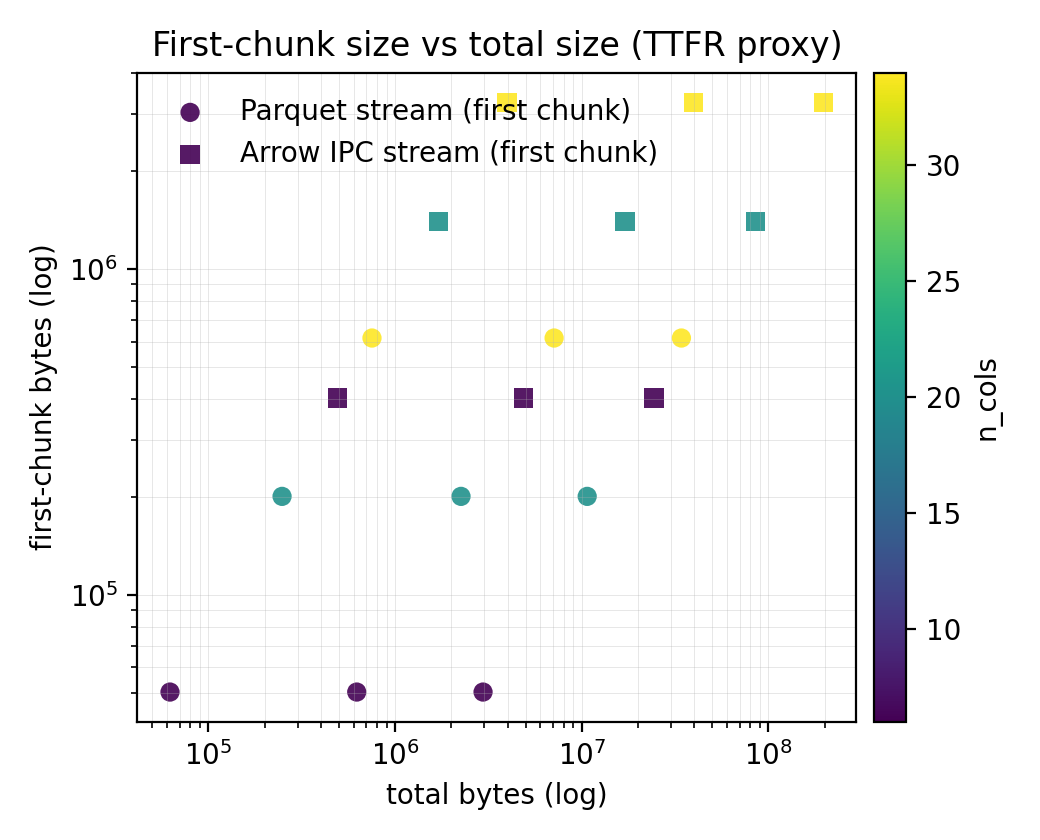
\includegraphics[width=\columnwidth]{figures/fig_A2_tpcds_first_chunk_bytes.png}
  \Description{Scatter plot of first-chunk bytes versus total bytes for Parquet and Arrow IPC streaming, with color indicating column count. First chunks are much smaller than totals for large payloads.}
  \caption{TTFR proxy: first-chunk bytes vs.\ total bytes for streaming formats. Smaller first chunks enable faster time-to-first-rows and early-stop behaviors.}
  \label{fig:firstChunkVsTotal}
\end{figure}

\subsection{Decode proxy calibration}
To support \texttt{min\_latency} selection beyond pure ``min bytes'', we calibrate a simple decode proxy: nanoseconds per byte for decoding representative payloads. Figure~\ref{fig:decodeProxy} shows median decode ns/byte (IQR) for JSON, Parquet blob, and Arrow IPC blob on TPC-DS slices. As expected, Arrow IPC decodes substantially faster in Arrow-native stacks, while Parquet trades some decode cost for wire size.

\begin{figure}[t]
  \centering
  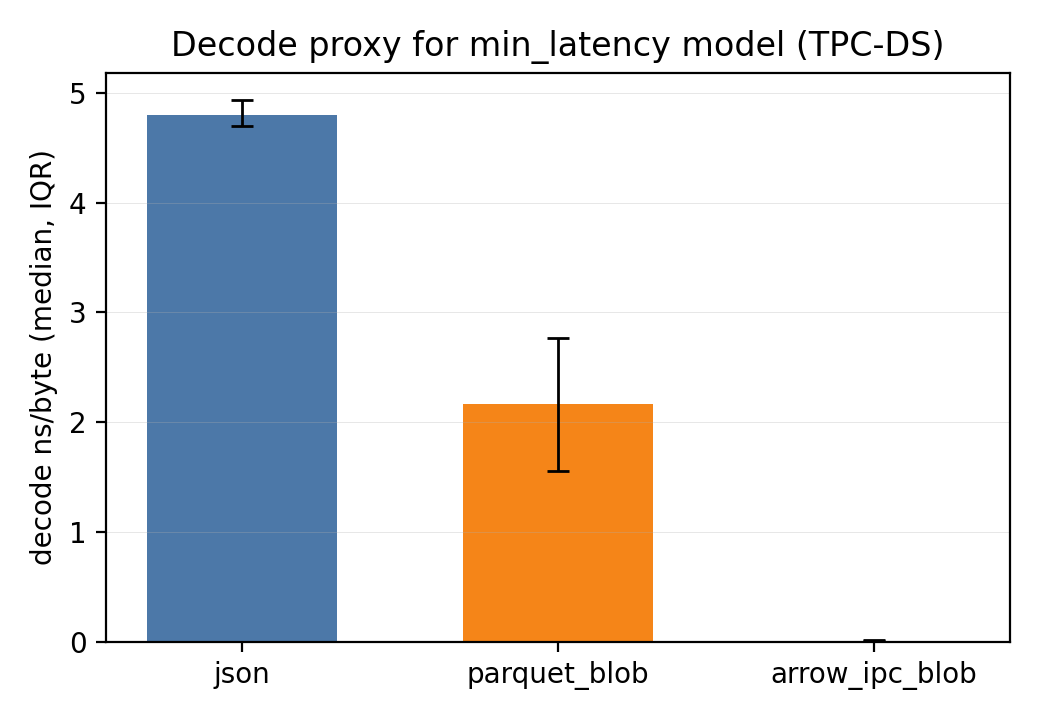
\includegraphics[width=0.85\columnwidth]{figures/fig_A3_tpcds_decode_ns_per_byte.png}
  \Description{Bar chart of decode nanoseconds per byte (median with IQR) for JSON, Parquet blob, and Arrow IPC blob. Arrow IPC shows near-zero decode cost per byte compared to the others.}
  \caption{Decode proxy calibration (TPC-DS): median decode ns/byte (IQR) for JSON, Parquet, and Arrow IPC. Used as an optional term in \texttt{min\_latency} scoring.}
  \label{fig:decodeProxy}
\end{figure}

\subsection{BIRD transport: bytes and latency on real workloads}
We evaluate \system on BIRD dev with \textbf{gold SQL} to isolate transport effects from NL2SQL quality. For each question, the client executes the reference SQL on the corresponding SQLite database, registers the materialized result once, and then compares two transport arms on the same result: (A) baseline ``JSON-only'' MCP delivery, and (B) enhanced delivery with hint-aware format choice and Parquet blob fetch when beneficial.

\smallskip
\noindent\textbf{Payload (wire bytes).}
On BIRD full dev (1534 queries), the aggregate wire volume decreases from 43{,}439{,}928 bytes (baseline JSON) to 6{,}386{,}514 bytes (enhanced selection), a 6.8$\times$ reduction. Medians remain small (57 bytes) because many queries return tiny results; p95 bytes decreases from 11{,}966 to 3{,}650, and the enhanced arm chooses Parquet for 164/1534 queries, concentrating savings on the tail.

\smallskip
\noindent\textbf{Latency and overhead.}
Figure~\ref{fig:birdLatencyPaired} plots per-query variant latency against baseline latency (paired). On localhost, the enhanced \emph{single fetch} remains comparable to baseline fetch because the dominant effect is network loopback; the primary overhead is the additional ``describe'' call in client-driven selection. Figure~\ref{fig:birdOverheadBreakdown} breaks down median overhead, highlighting that one-shot server-side selection can remove the describe round-trip while retaining the data-plane benefits.

\begin{figure}[t]
  \centering
  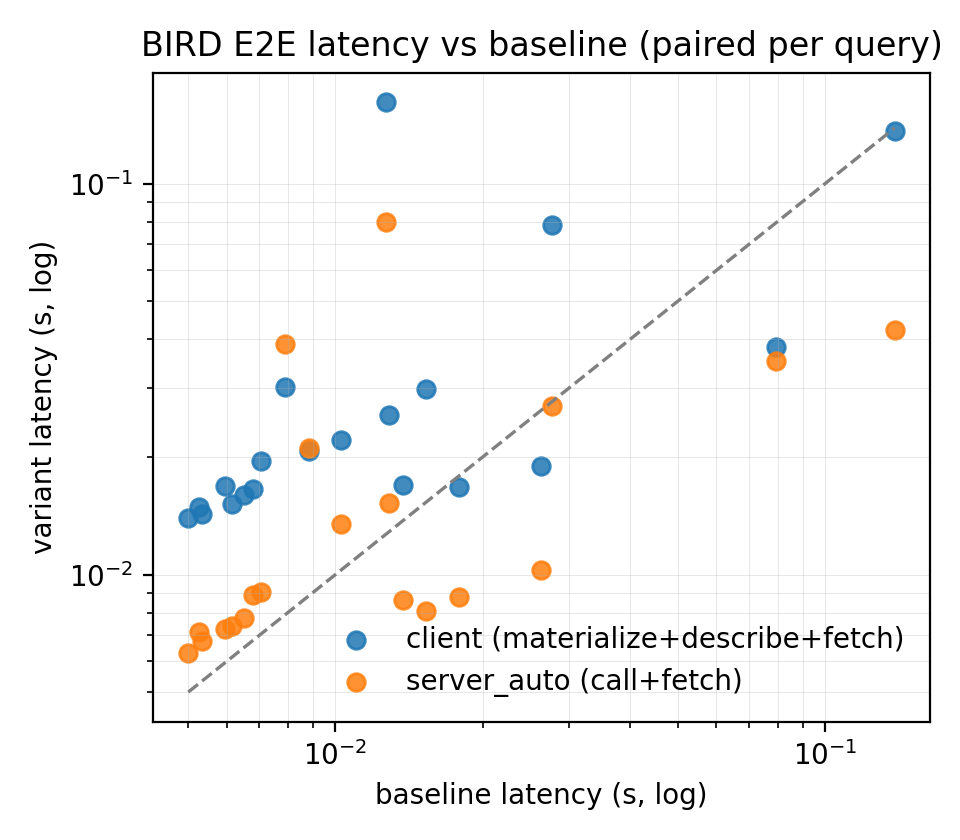
\includegraphics[width=\columnwidth]{figures/fig_B1_bird_latency_paired.png}
  \Description{Paired scatter plot on log-log axes comparing per-query variant latency against baseline latency for client selection and server-side auto selection. A diagonal reference line indicates parity.}
  \caption{BIRD paired per-query latency: client-driven selection (materialize+describe+fetch) and one-shot server-side selection (call+fetch) compared to baseline (JSON fetch). Both axes are log-scaled seconds.}
  \label{fig:birdLatencyPaired}
\end{figure}

\begin{figure}[t]
  \centering
  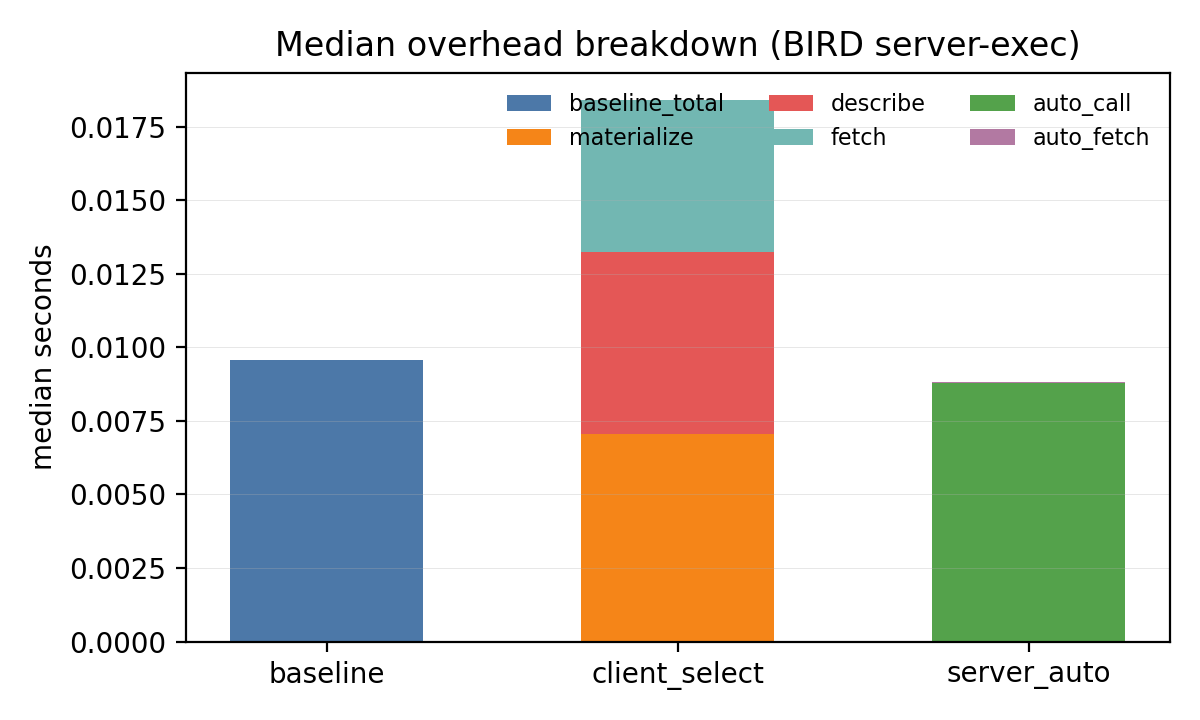
\includegraphics[width=\columnwidth]{figures/fig_B3_bird_overhead_breakdown.png}
  \Description{Stacked bar chart breaking down median overhead in seconds for baseline, client selection, and server auto. Client selection includes materialize, describe, and fetch components.}
  \caption{Median overhead breakdown on BIRD: baseline total vs.\ client selection (materialize, describe, fetch) vs.\ server-side one-shot selection.}
  \label{fig:birdOverheadBreakdown}
\end{figure}

\subsection{Codec/encoding trade-offs within Parquet}
Within the Parquet arm, codec choice trades off wire size against encode+decode time. Figure~\ref{fig:codecBytes} shows Parquet bytes for a representative TPC-DS-derived table under different codec/strategy settings. Figure~\ref{fig:codecTradeoff} plots encode+decode time versus bytes, illustrating a Pareto frontier: Zstd often reduces bytes more than Snappy at moderate CPU cost, while Gzip tends to be slower for similar or smaller gains.

\begin{figure}[t]
  \centering
  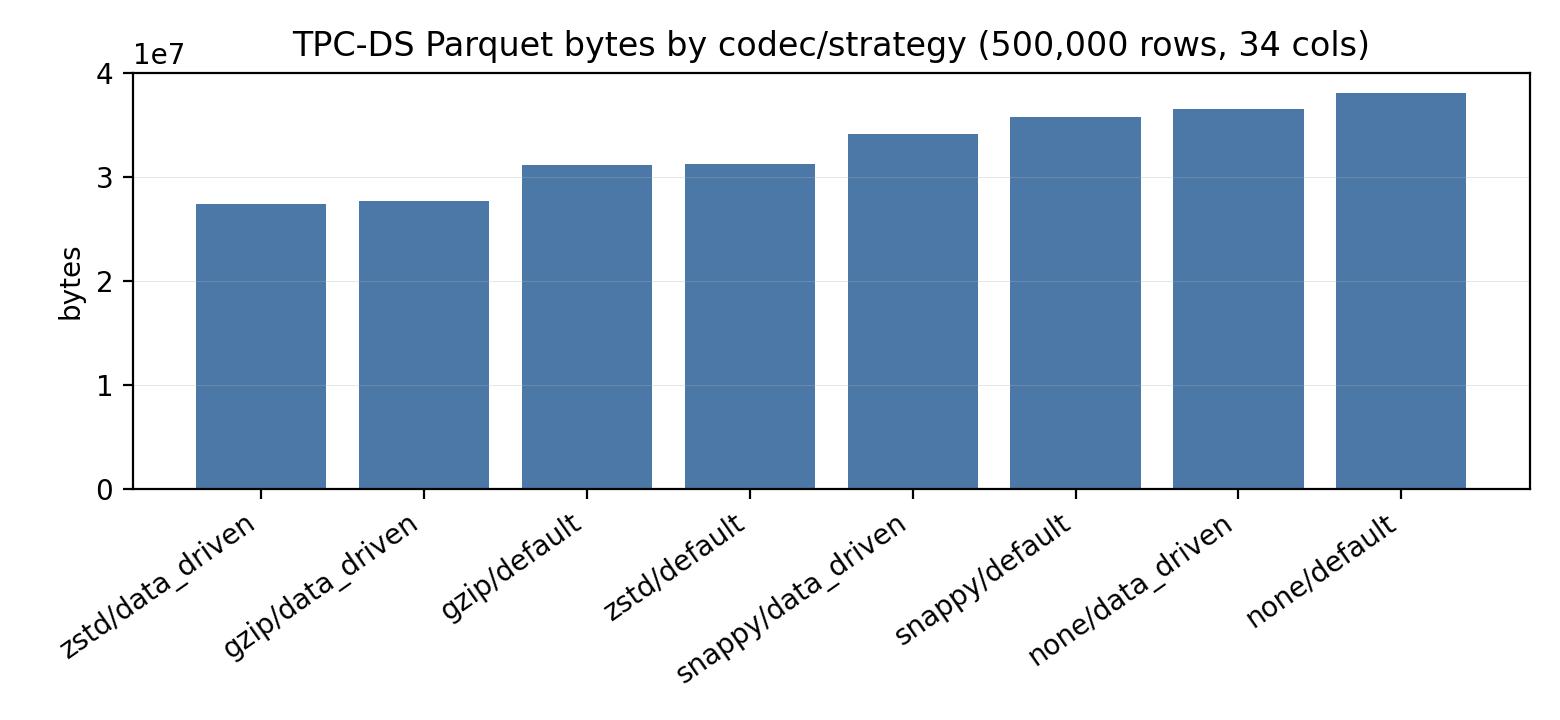
\includegraphics[width=\columnwidth]{figures/fig_C1_codec_bytes_bars.png}
  \Description{Bar chart comparing Parquet payload bytes across codec and encoding-strategy combinations for a fixed TPC-DS-derived table.}
  \caption{TPC-DS Parquet bytes by codec/strategy for a representative table.}
  \label{fig:codecBytes}
\end{figure}

\begin{figure}[t]
  \centering
  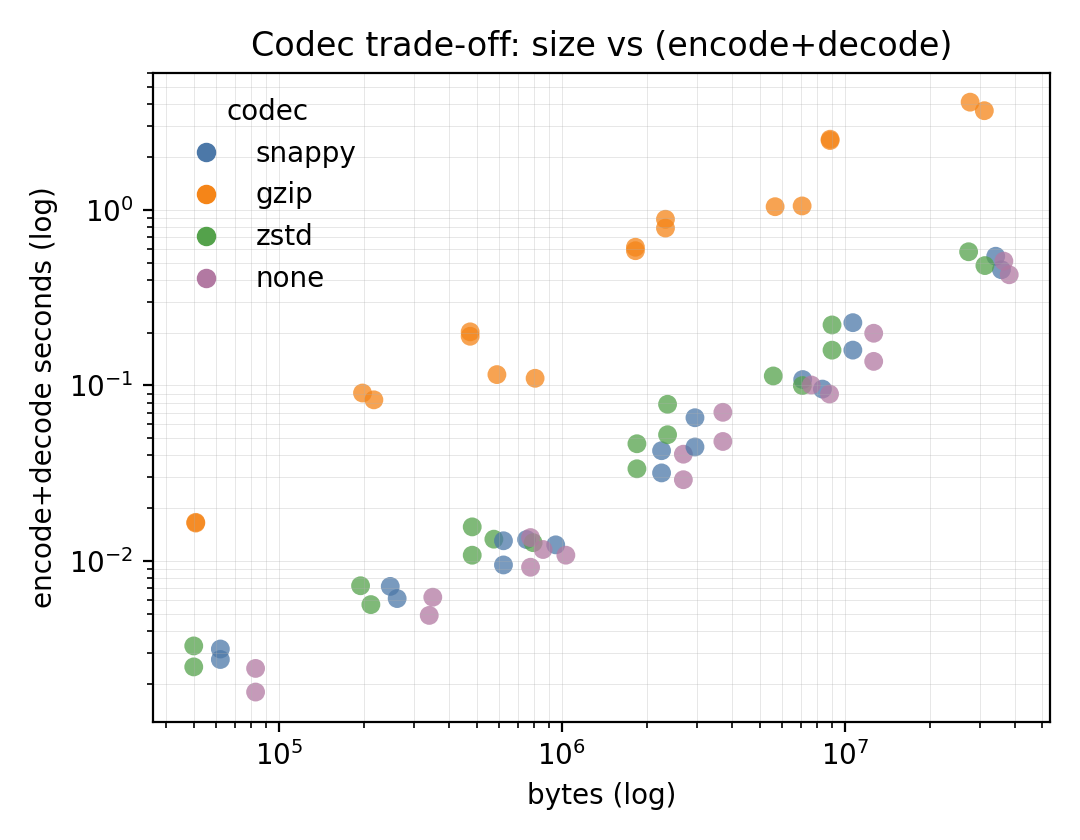
\includegraphics[width=\columnwidth]{figures/fig_C2_codec_tradeoff_scatter.png}
  \Description{Scatter plot on log-log axes showing encode+decode time versus payload bytes for multiple codecs. Points reveal size-latency trade-offs and a Pareto frontier.}
  \caption{Codec trade-off: payload size versus encode+decode time (log-log). Points illustrate the Pareto structure across codecs.}
  \label{fig:codecTradeoff}
\end{figure}

\subsection{Threats to validity}
\textbf{Localhost transport:} reported millisecond latencies reflect same-machine loopback and do not capture WAN RTT or bandwidth variability; payload ratios are more portable than absolute times. \textbf{Gold SQL isolation:} core BIRD runs execute reference SQL, isolating transport but not evaluating NL2SQL accuracy. \textbf{Result caps and caching:} benchmarks cap pathological result sizes and use pragmatic caching; we compare baseline and enhanced on the same materialized result ids to preserve fairness.

\section{Conclusion}
\label{sec:conclude}
AI agents increasingly rely on tool outputs as the substrate for reasoning, but existing MCP deployments frequently deliver large structured results through a JSON-RPC control plane that is ill-suited for tabular payloads. This paper presented \system, a dynamic format selection framework that splits MCP results into a small control-plane envelope (text plus a machine-readable descriptor) and a streamable HTTP data plane for large payload bytes. For tabular results, \system supports JSON records for compatibility and Parquet blob/stream delivery for efficient transfer, incremental consumption, and early termination; it further supports target-driven selection (min bytes, min latency, or min time-to-first-rows) and codec choices within Parquet.

Our evaluation on synthetic grids, TPC-DS slices, and BIRD dev query results shows that the design is practical and yields substantial reductions in aggregate wire volume versus JSON baselines, while preserving low millisecond-scale fetch latency on localhost. The results also highlight the importance of selection placement: client-driven selection benefits from explicit hints but incurs a ``describe'' overhead that can be removed via one-shot server-side selection.

\smallskip
\noindent\textbf{Limitations and future work.}
Our current benchmarks focus on localhost and fixed bandwidth assumptions; evaluating under realistic WAN conditions and varying congestion is an immediate next step. Second, while we treat unstructured outputs as first-class, richer multimodal payloads (e.g., images, embeddings, and mixed text+table outputs) require additional conventions for schema/typing and safe decoding. Third, selection policies can be made more data-driven: online learning can incorporate workload drift and privacy constraints, and codec selection can be extended beyond simple rule-based strategies. Finally, integrating end-to-end authorization, auditing, and privacy-preserving transformations into the data plane remains essential for multi-tenant streamable HTTP deployments.

\begin{acks}
This work was supported by the Department of Computer Science at Purdue University.
\end{acks}

\bibliographystyle{ACM-Reference-Format}
\bibliography{ref}

\end{document}
\endinput